\section{Secondary Groups}

%TODO: Explain format read from the Computer Vision group (and results if we manage to get some examples of their work), and output given to the Emotion Synthesis group
Our Secondary groups were Computer vision and Emotion Synthesis. Our task in final pipeline was to read the input given by CV group and send the output to ES group.

\subsection{Computer Vision Group}
%Format read from CV Group
After training our models with the Bosphorus database we need to predict an emotion by reading input given from CV group. They are giving input in numpy array containing $24$ landmarks. We did dimensionality reduction while training our model so we are using the same pca model to do the equal amount of dimensionality reduction for the given input. 

\subsection{Emotion Synthesis Group}
%Format given to Emotion Synthesis Group
We are using SVM model trained on bosphorus dataset as it's more stable and gives better accuracy as you saw in Implementation section. We are sending output in a json format contatining all the 6 labels with their confidence score which tells about the probability of the emotion predicted by our model. We are also sending confusion matrix of our model so that they can get the idea how well our model is performing for each of the labels.


\begin{figure}[H]
    \centering
    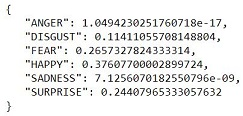
\includegraphics[height= 25mm]{figures/emotion_output.jpg}
    \caption{Output Format for ES Group}
    \label{emotion_output}
\end{figure}


%Reflection on how well the integration in the final pipeline worked
%what worked well
%what were challenges